\section{Montagem dos equipamentos}

Os equipamentos foram transportados em uma caixa de madeira, de aproximadamente
$0,6~m$ x $0,6~m$ x $0,6~m$, pesando ao todo aproximadamente $100~kg$. Algumas
ferramentas não previstas foram disponibilizadas pelo cliente. A lista de
ferramentas e equipamentos utilizados encontra-se a seguir:

\begin{itemize}
  \item $1\times$ \textit{Housing} para eletrônica embarcada
  \item $4\times$ Senores indutivos
  \item $1\times$ Cabo umbilical de $60m$
  \item $1\times$ Caixa hermética para eletrônica de superfície
  \item $1\times$ Tablet com interface para operação
  \item $2\times$ Conjuntos de fixação para sensores indutivos ($1x$ aço AISI
  $1020$ e $1\times$ aço inoxidável)
  \item $3\times$ Abraçadeira metálicas para fixação do \textit{housing}
  \item $1\times$ Conjunto de abraçadeiras de velcro para fixação dos cabos
  \item $1\times$ Fita dupla-face para posicionamento dos sensores
  \item $1\times$ Caneta para marcação do posicionamento para solda dos
  fixadores
 \end{itemize}
 
 A montagem dos equipamentos ocorreu no espaço próximo ao stoplog que seria
 realizada a demonstração. Primeiro montou-se o \textit{housing} na face
 superior da Viga, no lado direito (perspectiva do operador) e então foram
 posicionados os sensores indutivos, buscando-se a melhor distância em relação à
 face de interesse da chave da Viga Pescadora. Neste ponto, constatou-se que o
 cabo de alimentação do sensor da chave, do lado direito, era curto. Mudou-se o
 lado de fixação do \textit{housing} para a esquerda da viga, o que solucionou o problema.
 
\begin{figure}[h]
\centering
	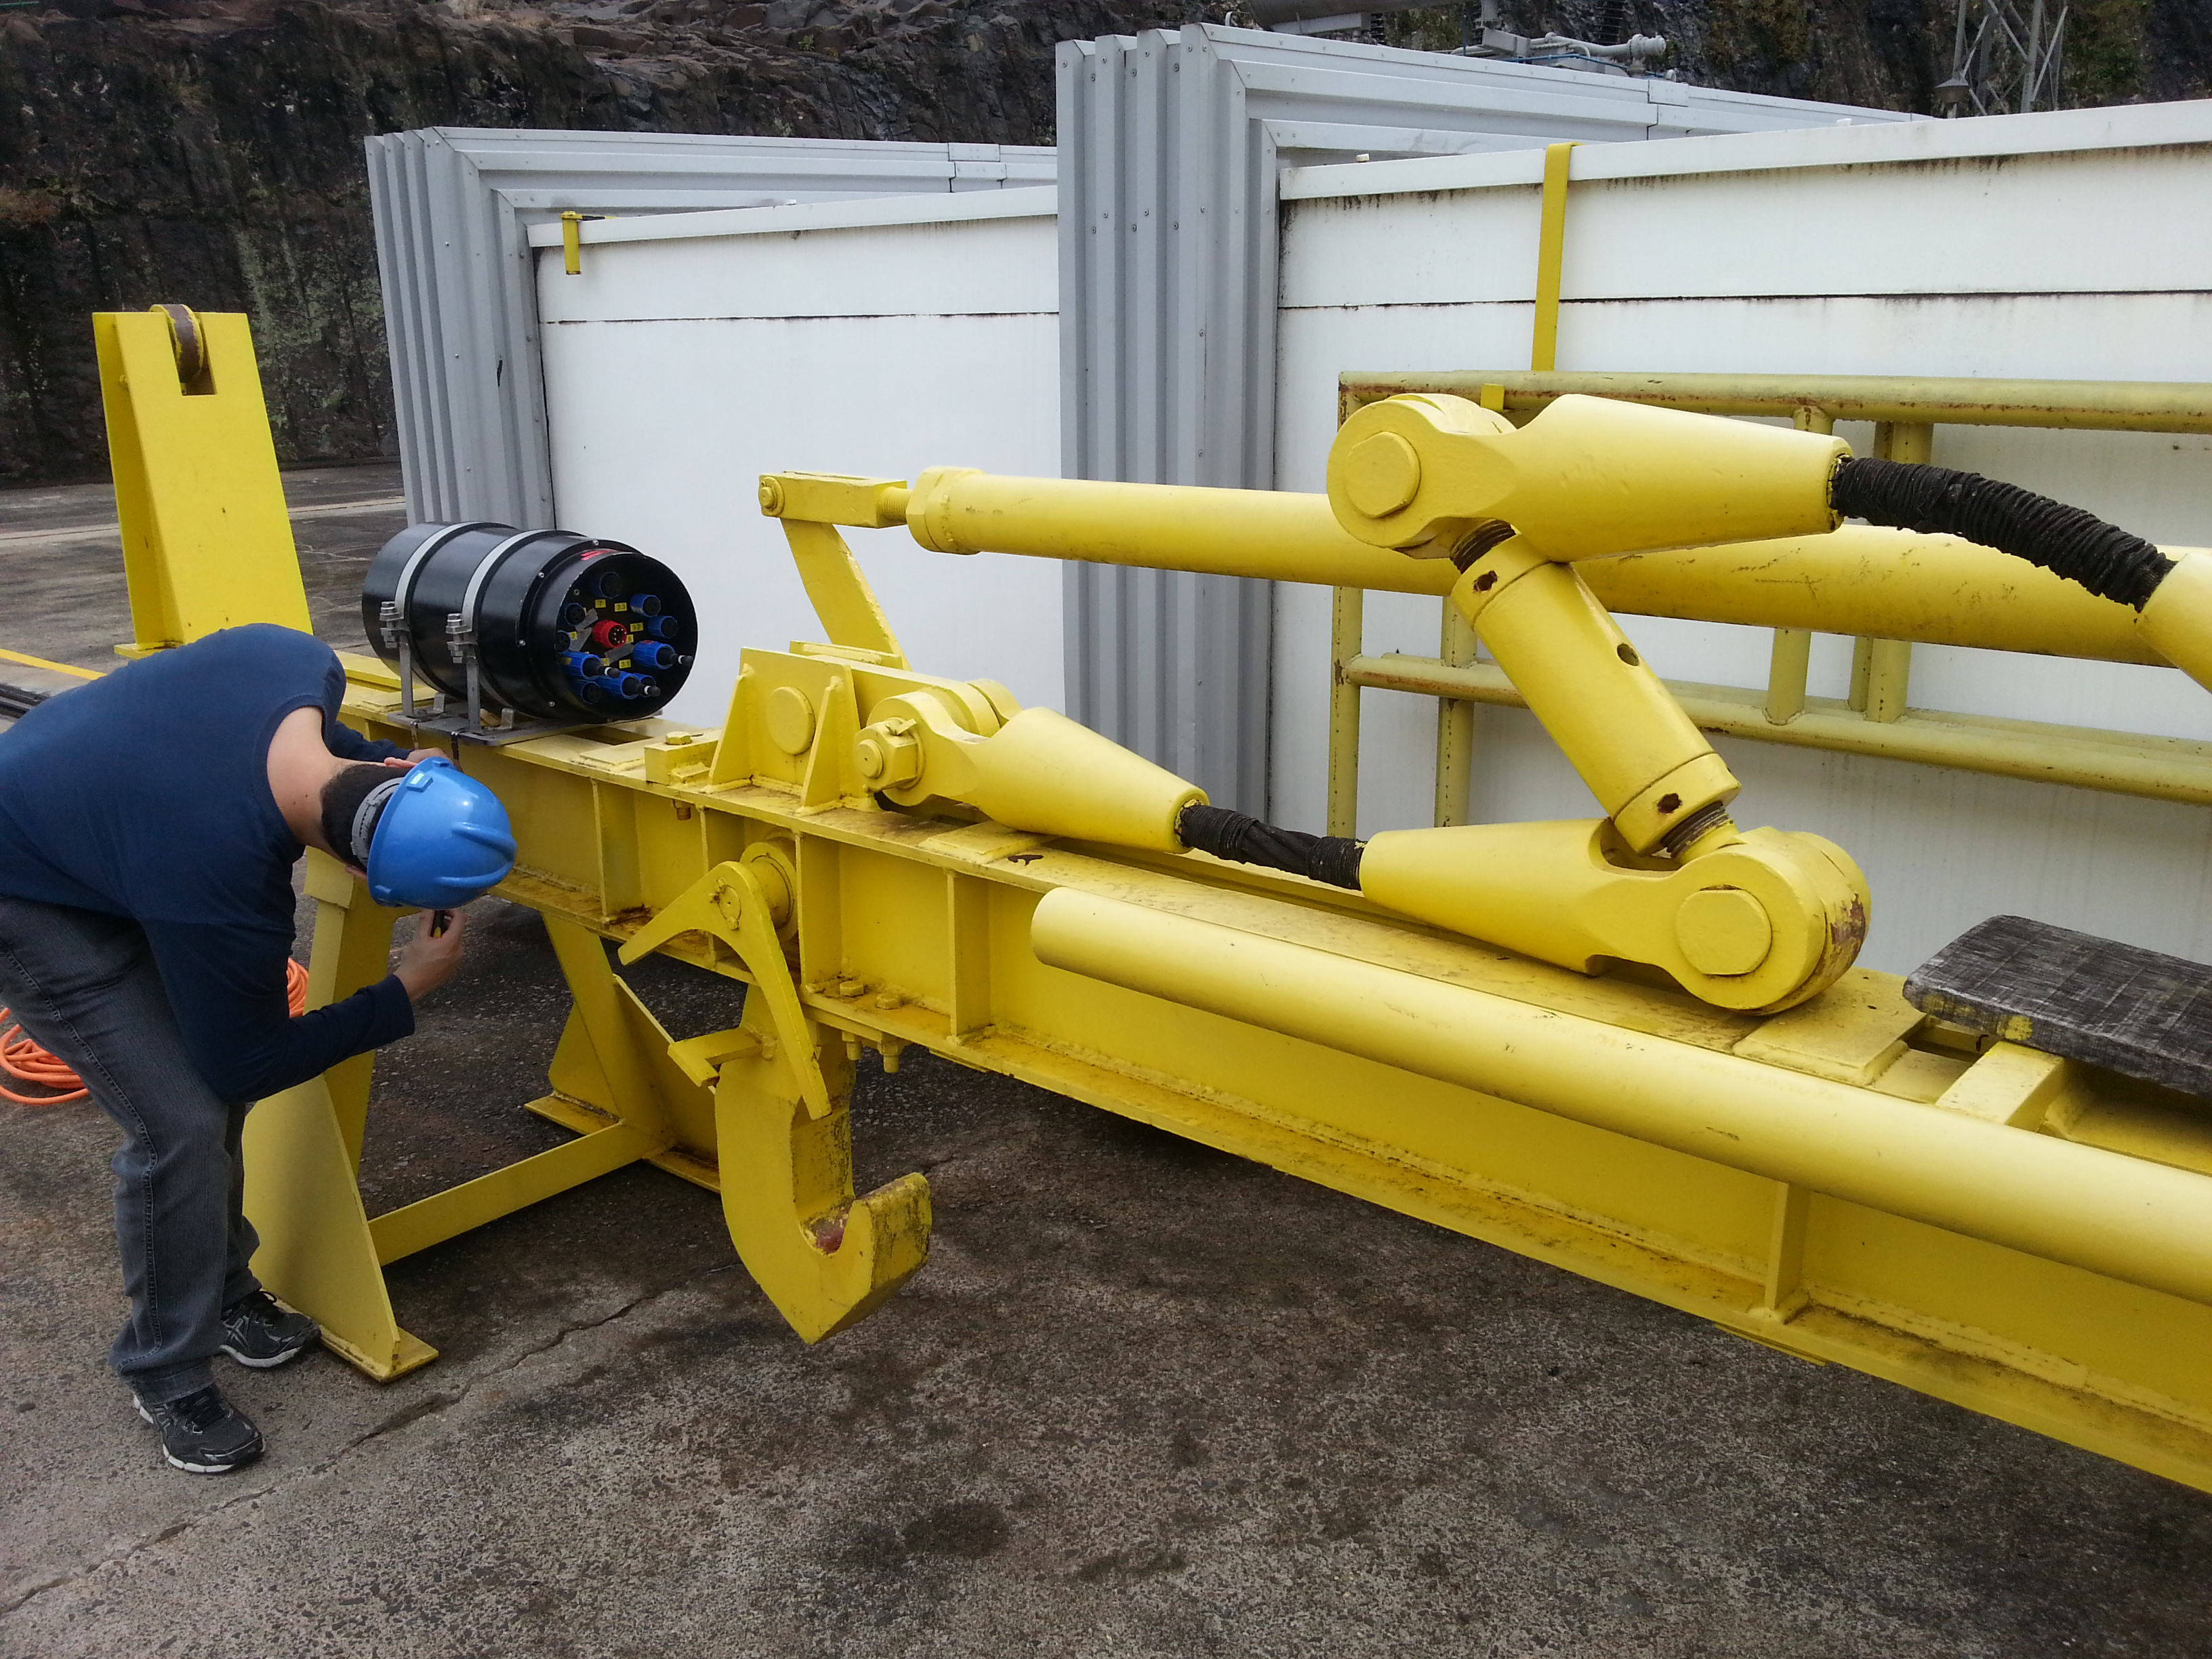
\includegraphics[width=0.9\columnwidth]{figs/housing_montagem}
	\caption{Montagem do \textit{Housing} na Viga Pescadora}
	\label{fig::housing_montagem}
\end{figure}
 
 Para os sensores da garra, foi utilizada uma fita dupla-face
 para auxiliar na investigação do melhor posicionamento dos sensores, garantindo
 a detecção e também que não haveria contato físico do sensor com o olhal do
 stoplog.
 
\begin{figure}[h!]
\centering
	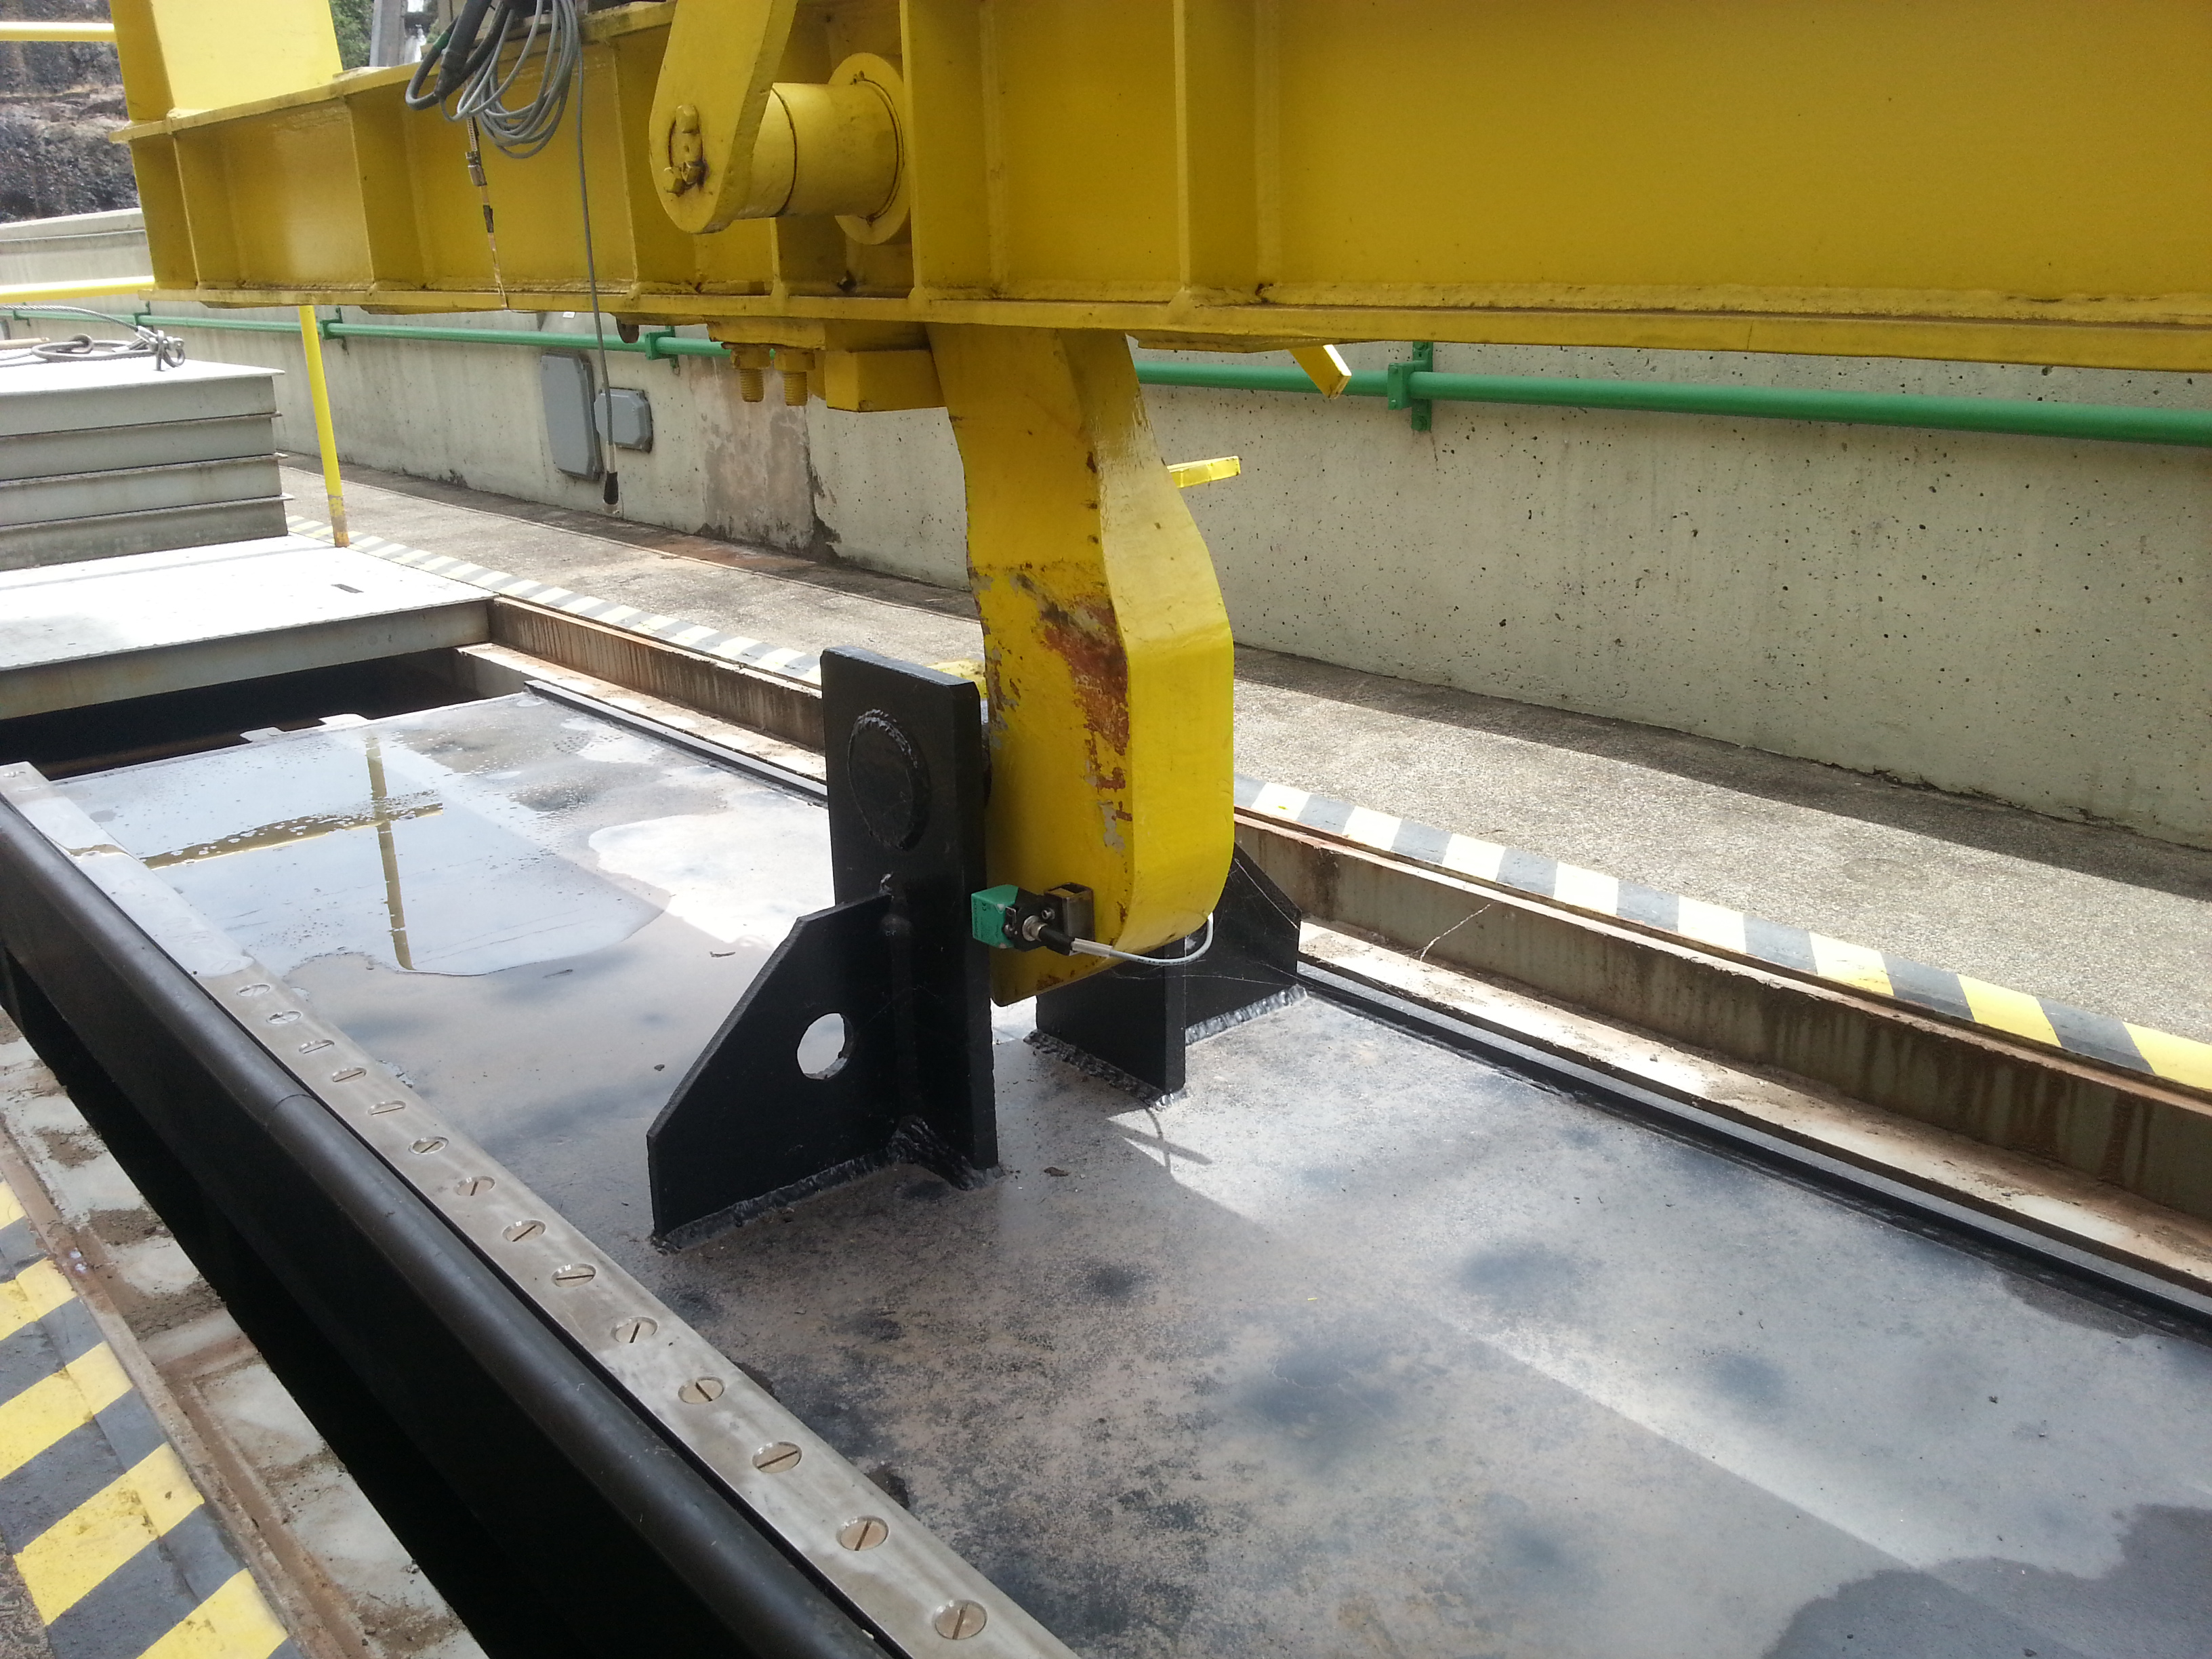
\includegraphics[width=0.9\columnwidth]{figs/sensor_olhal}
	\caption{Posição do sensor da garra e olhal}
	\label{fig::sensor_olhal}
\end{figure}

\begin{figure}[h!]
\centering
	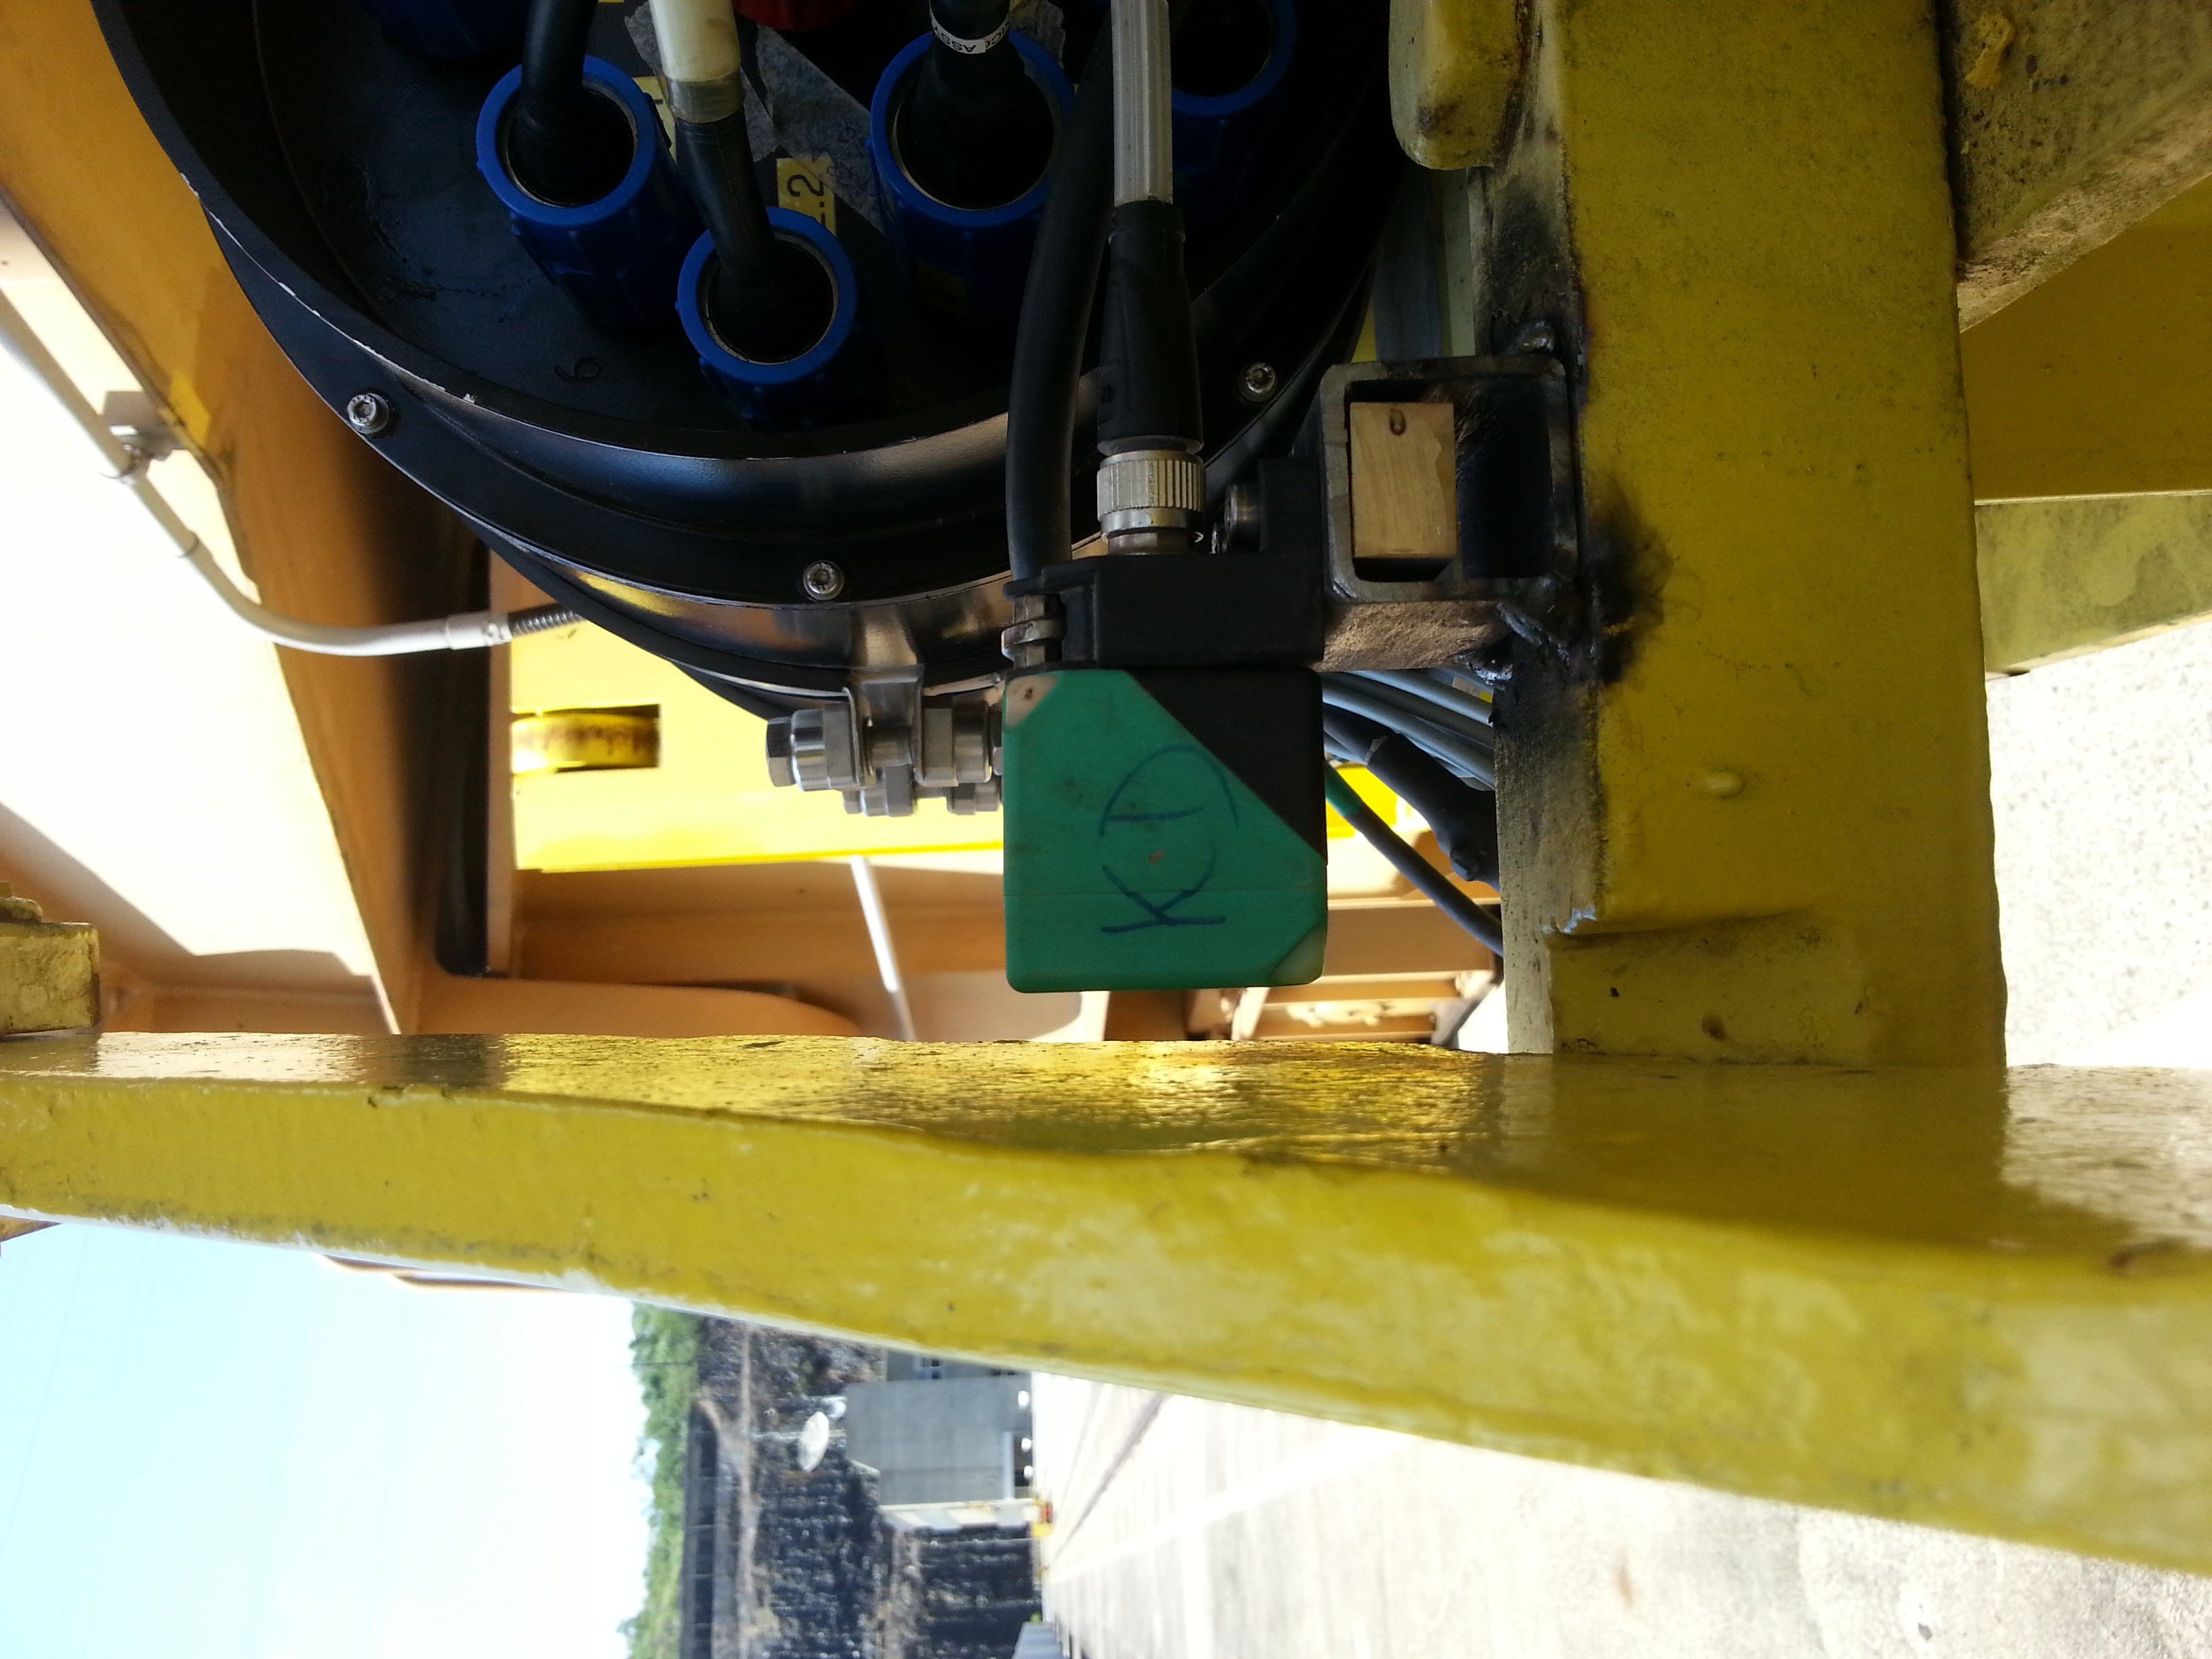
\includegraphics[width=0.7\columnwidth, angle=270]{figs/dist_sensor}
	\caption{Distância ótima do sensor para a chave}
	\label{fig::dist_sensor}
\end{figure}
 
 O procedimento de montagem dos equipamentos foi auxiliado pelos técnicos da
 usina, no local, fornecendo energia e ferramentas para facilitar a montagem.
 Também foi disponibilizado um técnico para a soldagem dos fixadores do sensor
 indutivo na viga.
 
 Posicionados os sensores, o técnico optou pela solda dos fixadores de aço
 carbono comum visto a maior facilidade de soldar este material, em relação ao
 conjunto de aço inoxidável. As peças foram deixadas para resfriamento natural
 até os sensores poderem ser montados nos fixadores.
 
 Os cabos foram fixados ao longo da viga, sem um posicionamento objetivo, sendo
 amarrado com a utlização de abraçadeiras de velcro e de plástico, esta última
 fornecidas pelo cliente. 
 
\begin{figure}[h!]
\centering
	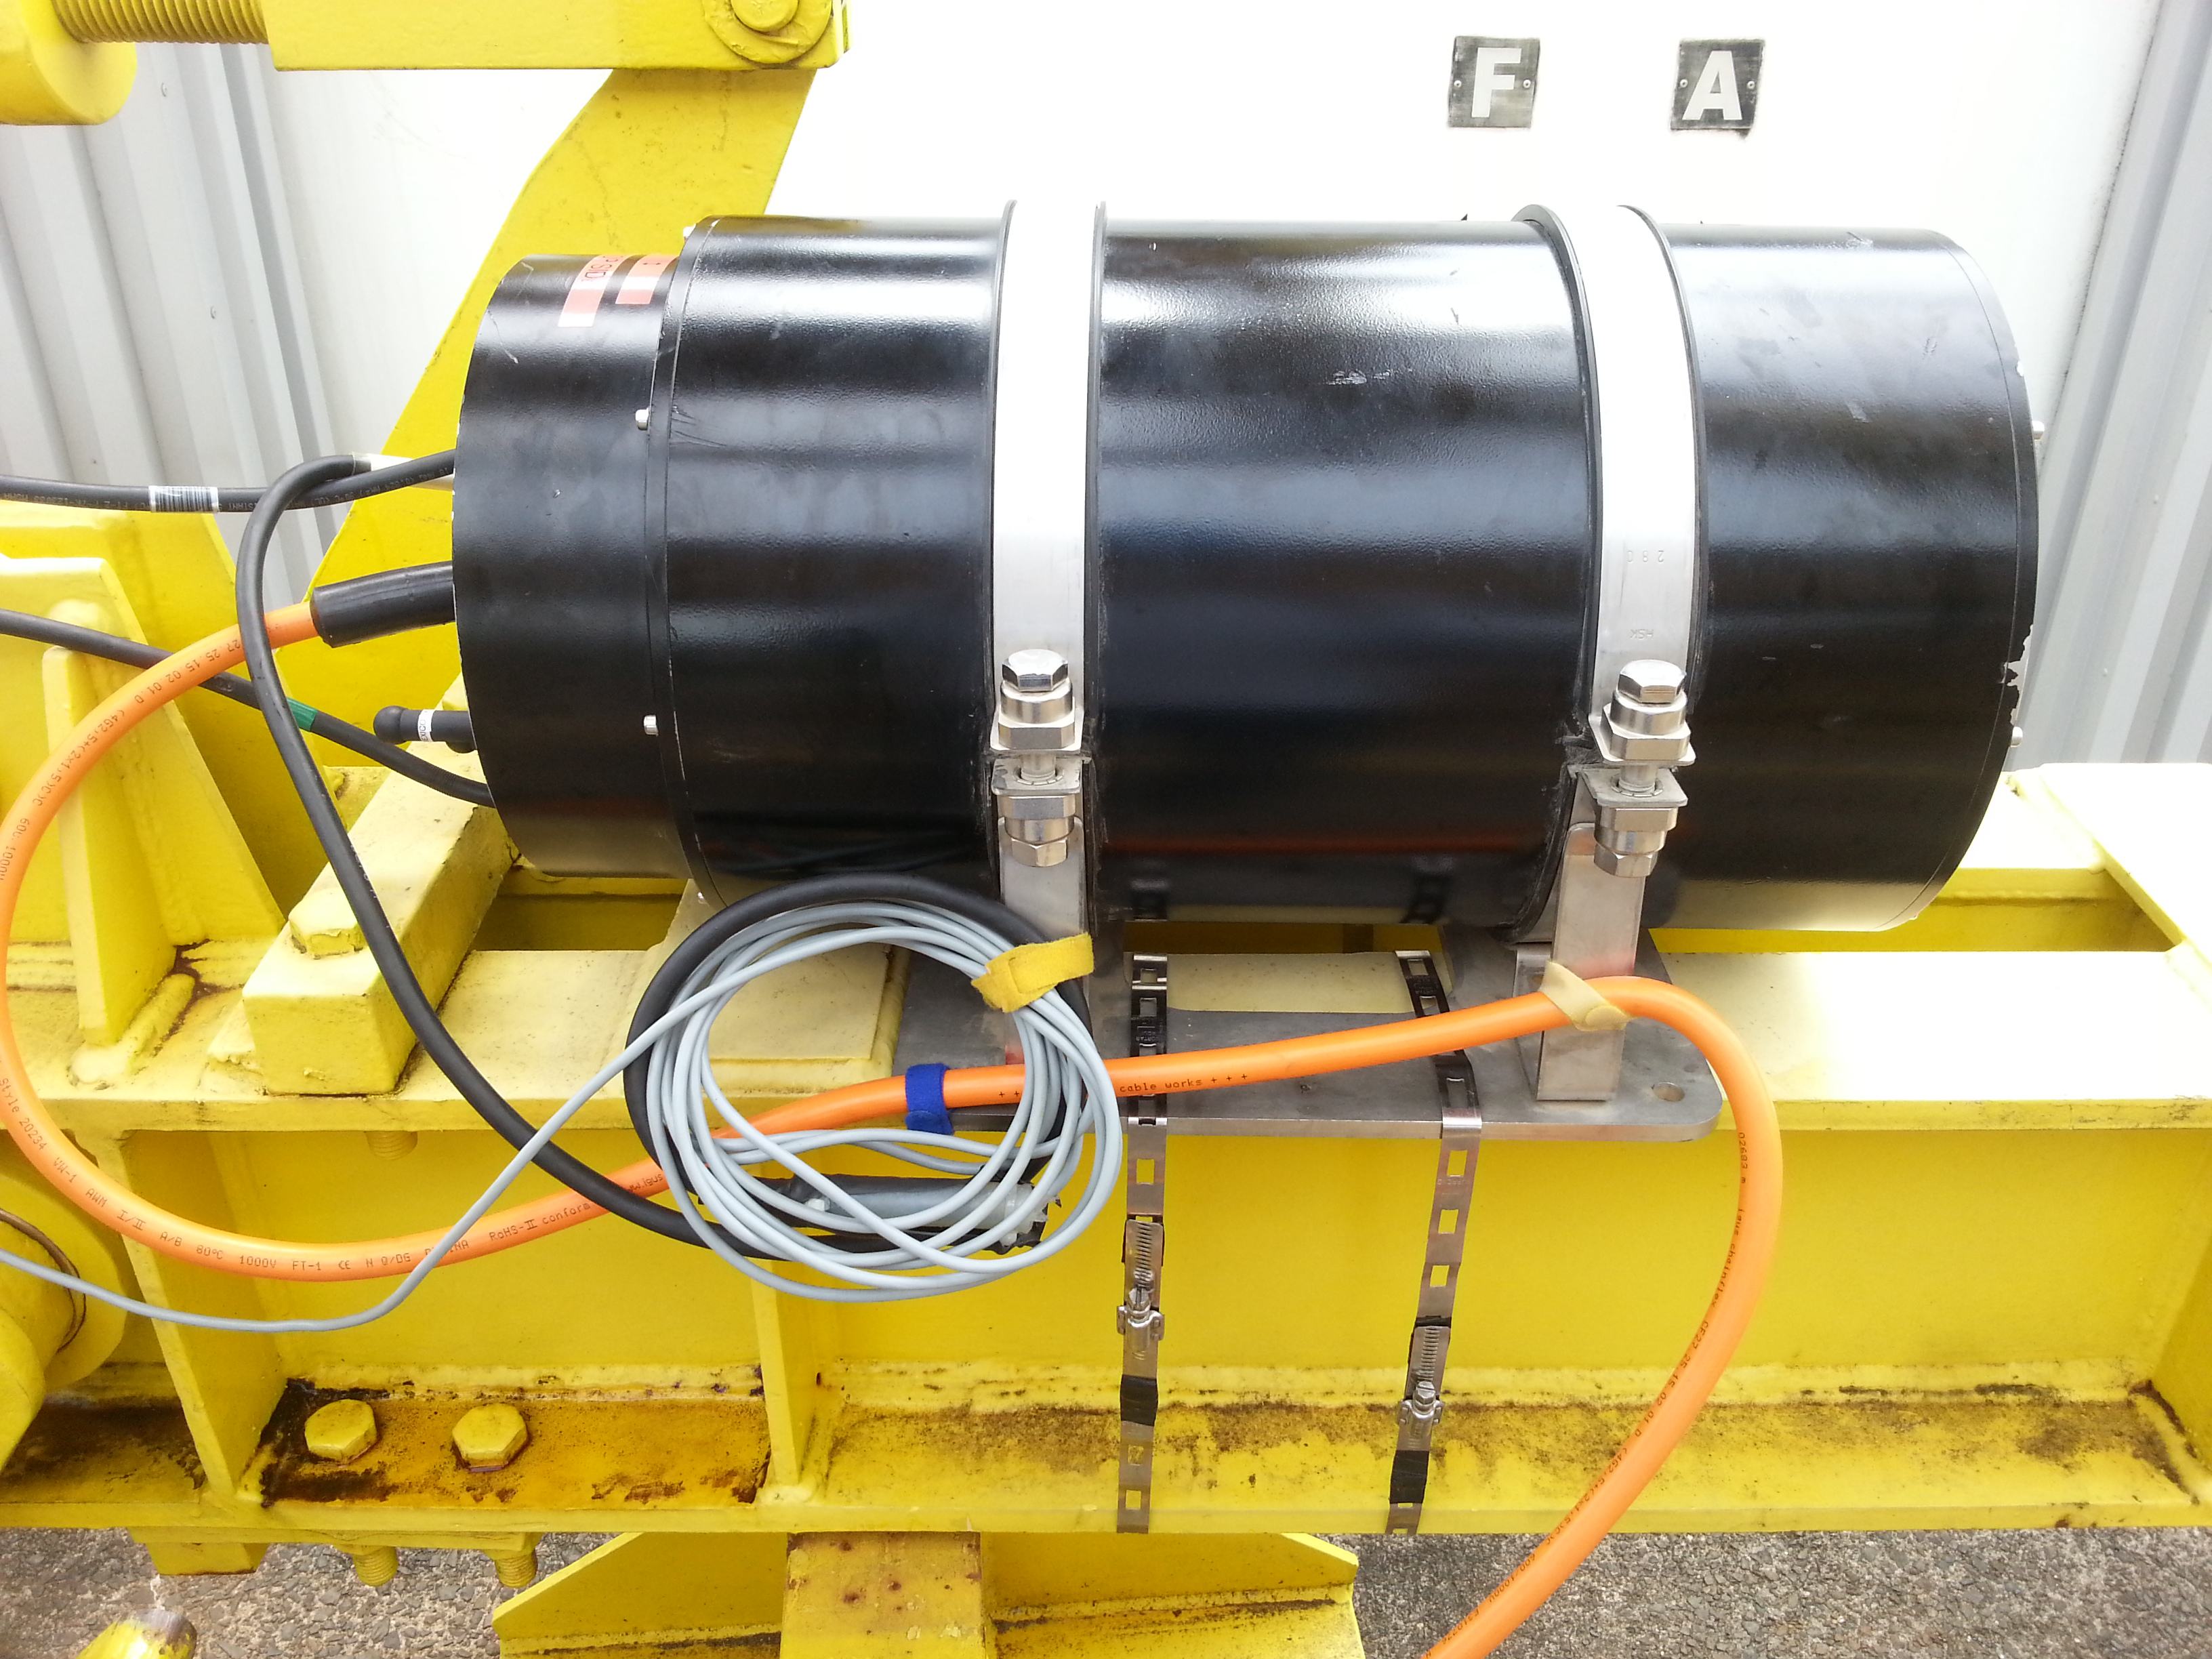
\includegraphics[width=0.8\columnwidth]{figs/fix_cabos}
	\caption{Fixação dos cabos e do \textit{Housing}}
	\label{fig::fix_cabos}
\end{figure} 

\begin{figure}[h!]
\centering
	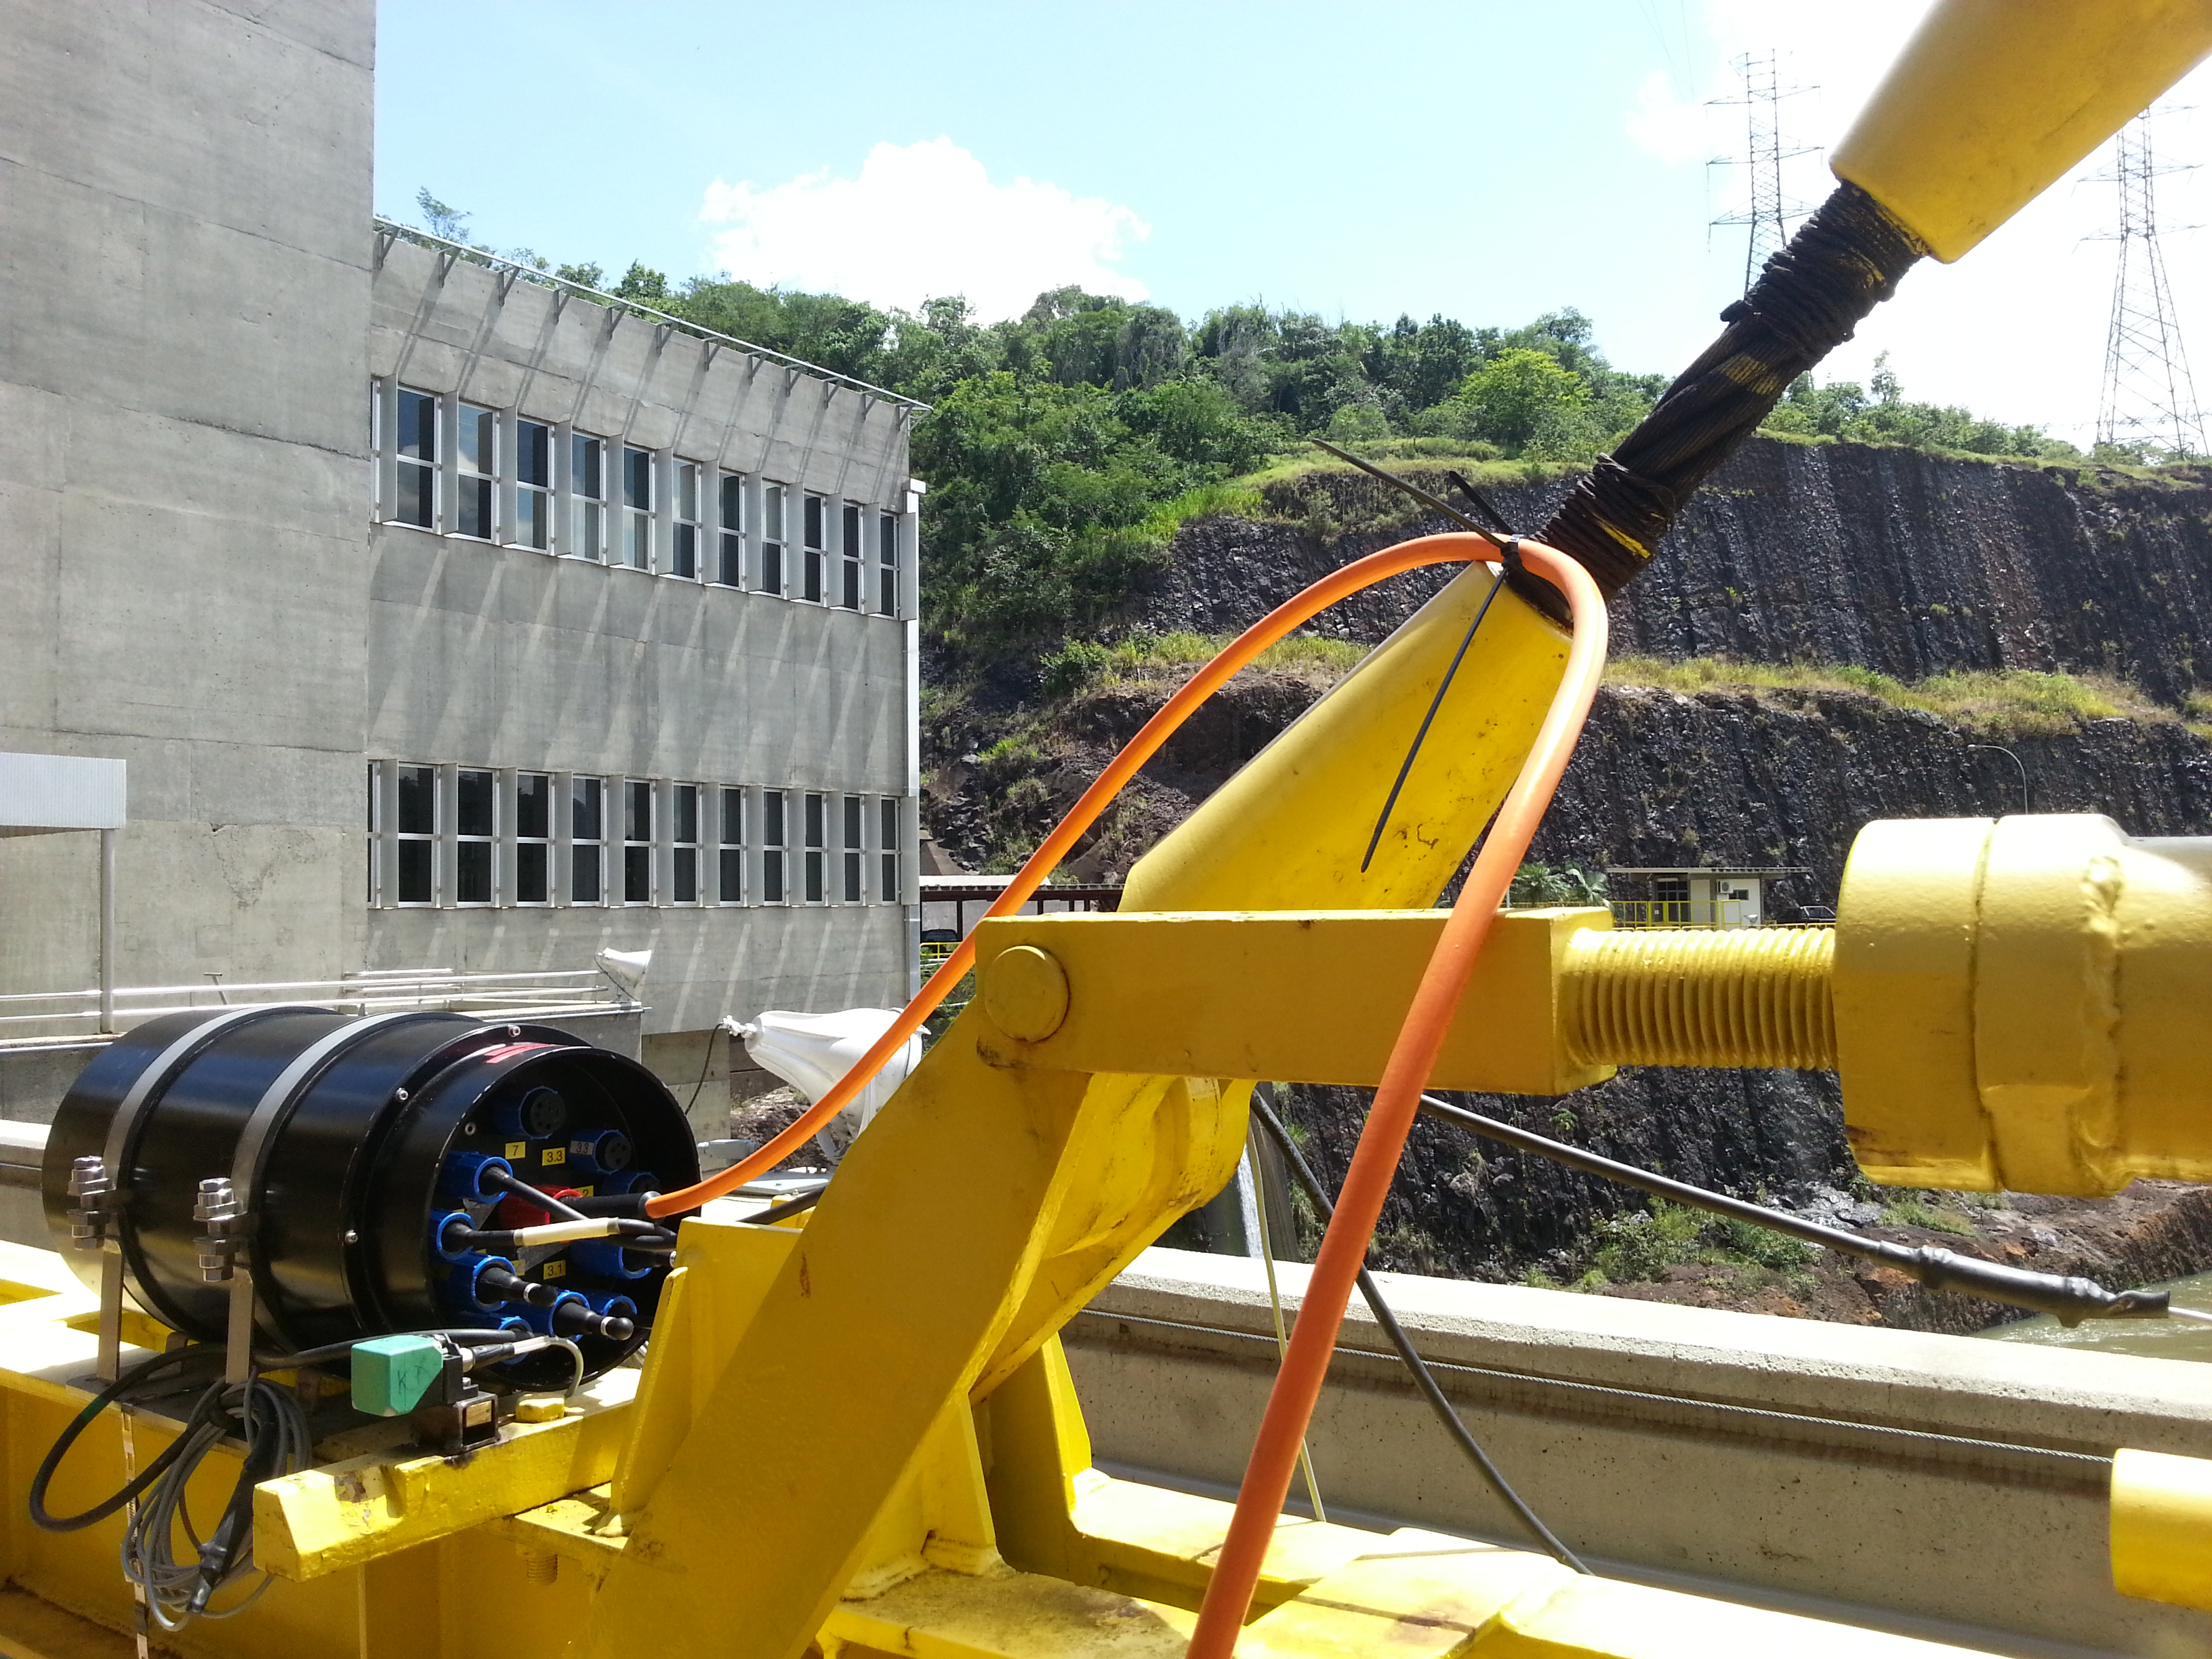
\includegraphics[width=0.8\columnwidth]{figs/fix_umbilical}
	\caption{Fixação do cabo umbilical na Viga Pescadora}
	\label{fig::fix_umbilical}
\end{figure} 
 
 A caixa de eletônica de superfície ficou localizada próxima a ponte rolante,
 sendo alimentada por uma extensão fornecida pelo cliente, e ligada a rede da
 usina. O operador do pórtico ficou de posse do tablet, sendo orientado pelo
 Renan Freitas durante a operação.
